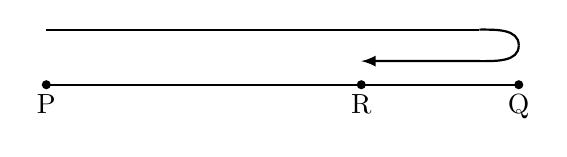
\begin{tikzpicture}
%\draw [help lines, color=lightgray] (0,0) grid (6,2);
\draw [thick] (0,1) coordinate (init) node [below] {P} -- (6,1) coordinate (med) node [below] {Q} -- (4,1) coordinate (fin) node [below] {R}; ;
\draw [thick] (0,1.7)  to (5.5,1.7);
\draw [thick] (5.5,1.7) to  [out=0,in=90] (6,1.5);
\draw [thick,-latex] (6,1.5) to  [out=270,in=0] (5.5,1.3) to (4,1.3);
\draw [fill=black]  (init) circle [radius=0.05];
\draw [fill=black]  (med) circle [radius=0.05];
\draw [fill=black]  (fin) circle [radius=0.05];

\end{tikzpicture}